\chapter{ASLA}

\begin{figure}
	\centering
	\centerline{
		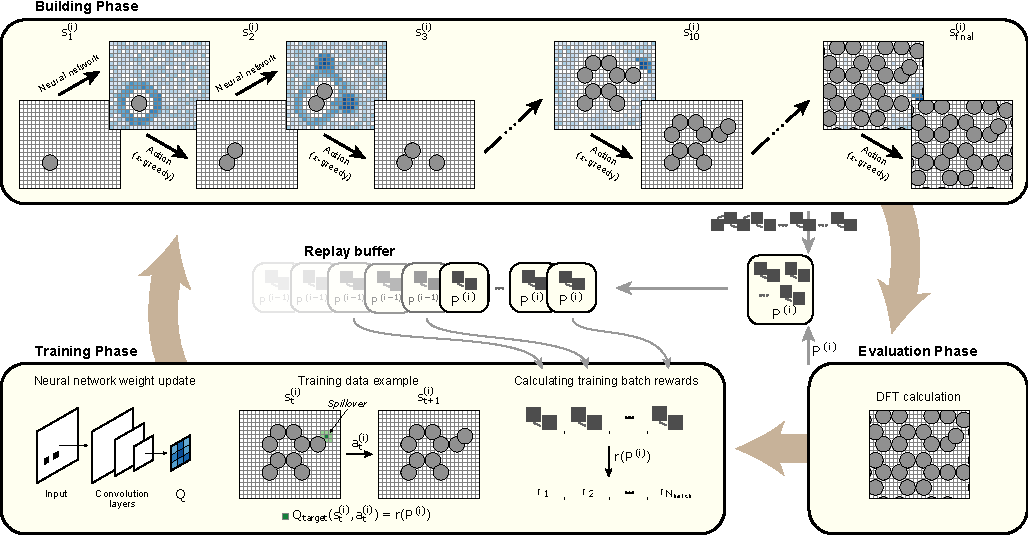
\includegraphics[width=1.3\columnwidth]{graphics/ASLA_overview.pdf}
	}
	\captionsetup{width=1.3\columnwidth}
	\caption{Overview of the three phases in ASLA. For each step $t$ in the building phase of episode $i$, the current grid $s_t^{(i)}$ is inputted into the CNN, which outputs the Q-values of each gridpoint. Depending on the current build policy, an action $a_t^{(i)}$ is taken, placing an atom on the chosen grid point. This step is repeated until all atoms are placed. The completed structure $s_{final}^{(i)}$ is then passed onto the evaluation phase, where the property $\mathcal{P}^{(i)}$ is calculated (e.g. a DFT energy calculation). The results from the evaluation phase are then saved in the Replay Buffer, storing state-action pairs and their associated property. During the training phase, a number of state-action pairs are loaded from the replay buffer and used to train the CNN using backpropagation to improve future Q-value estimates. The illustration is taken from \cite{Hammer}.}
	\label{fig:ASLA_overview}
\end{figure}

The Atomistic Structure Learning Algorithm (ASLA) aims to build atomic structures that optimize some property $\mathcal{P}$ \cite{Hammer}. ASLA is modelled as an MDP: The atoms it places on its board are converted to a reward, which ASLA will try to maximize \cite{henrik_DLA}. ASLA will estimate where on the 'board' to place the next atom by analyzing the current board with a CNN, which outputs a value at each point on the board, indicating the estimated reward for putting the next atom there. An instance of ASLA (\textit{agent}) works through 3 phases when building a new structure: The \textit{building} phase, the \textit{evaluation} phase and the \textit{training} phase. An overview of each of these phases can be seen on figure \ref{fig:ASLA_overview}.\\

In this project, ASLA will have one half of a benzene ring as a template and will search for optimal structures by placing additional 3 $C$ and 3 $H$ atoms. The property $\mathcal{P}$ that ASLA will try to optimize is in this case the potential energy. The optimal structure using a $C_6H_6$-setup is the benzene ring, resulting in a global minimum in potential energy of around $\SI{-70.17}{\electronvolt}$.

\section{Building phase}
During the building phase, the agent will use its current knowledge to estimate where to place atom $t$ ($a_t$) given the current state of the 'board' ($s_t$), called a \textit{grid}. The agent can only place atoms at discrete points on the grid, and at least one atom is prepositioned on the it as a starting point for the agent (a \textit{template}) \cite{henrik_DLA}. 

% Q-values
The agent awards each point on the grid some value (Q-value) between $-1$ and $1$ \cite{henrik_DLA}. This value is the agents current estimate for the final reward of the complete structure if an atom is placed on that grid point. These Q-values are calculated using a CNN on the grid $s_t$ \cite{Hammer}. Based on the current build-policy, a grid point is chosen and an atom is placed there. This step is repeated until there are no more atoms left to place (an \textit{episode}). \\

% Building policies
To choose where to place the next atom, the agent has a \textit{build policy} for each episode. The build policy used by ASLA is a modified $\epsilon$-greedy policy with 2 parameters $\epsilon_\nu$ and $\epsilon_0$, both being small numbers less than $1$ \cite{henrik_DLA}. In the $\epsilon_\nu$-fraction of times, the agent chooses a random grid point among the $\nu$-fraction of highest Q-values. During the $\epsilon_0$-fraction of times, the point is chosen randomly between \textit{all} available points on the grid. During the remaining cases with probability $1-\epsilon_\nu - \epsilon_0$ the point with the highest Q-value is chosen (\textit{greedy} action). The parameters $\epsilon_\nu$ and $\epsilon_0$ implemented to encourage exploration of the grid in two different ways \cite{henrik_DLA}. The completely random action with probability $\epsilon_0$ attempts to encourage placing atoms at seemingly sub-optimal points in the hopes that the agent will find an even better structure than if it had chosen optimal points. The downside of this type of action is that getting out of a local minimum often requires several seemingly sub-optimal moves, which is not very likely to happen randomly. The $\epsilon_\nu$ moves were introduced to counter this downside by avoiding grid points that are obviously bad choices (eg. too close to another atom) and instead choosing among points that the agent has found potentially rewarding \cite{henrik_DLA}.


\section{Evaluation Phase}
A structure is evaluated after it has been completed by the builder. The value of the target parameter $\mathcal{P}^{(i)}$ is then calculated using the property function $P(s^{(i)}_{final})$ \cite{Hammer}. The goal could be to make the thermodynamically most stable structure at $T=0K$, in which case the parameter $\mathcal{P}$ would be the potential energy. The potential energy of a structure is calculated using density function theory (DFT), which is a computationally expensive quantum mechanical calculation \cite{henrik_DLA}.

After the DFT calculation, the energy, along the structure and each step of the building process is saved in the replay buffer. 

\section{Replay buffer}

Previous state-action pairs are stored in the replay buffer. Each of these pairs has an associated property value that comes from the structure with the best property value that was built using that state-action pair \cite{henrik_DLA}. During training, a batch of previous state action pairs are loaded from the replay buffer, the number of pairs being a parameter in ASLA \cite{henrik_DLA}. Included in the training batch is always the best structure ever made and some fraction of the most recent pairs as including these has a positive impact on the performance of the algorithm \cite{henrik_DLA}.


\section{Training phase}

During the training phase, a batch of state-action pairs $(s^{(i)}_t, a^{(i)}_t)$ from previous episodes $i$ are loaded from the replay buffer. Using these pairs, the CNN parameters are updated in a step called backpropagation. During this step, the root mean square error between the predicted Q-values and $Q_{target}$-values is minimized. The $Q_{target}$-values are calculated using the update rule \cite{Hammer}:
\begin{equation}
Q_{target}(s_t^{(i)}, a_t^{(i)}) = r(\mathcal{P}^{(i)})
\label{eq:update_rule}
\end{equation}
with $r\in [-1, 1]$ is the reward of episode $i$.

Furthermore, the training structures are rotated so that the CNN is taught rotational invariance. Lastly, to better simulate a continues potential energy surface, the Q-values from the backpropagation phase are smeared out to also affect nearby grid points , which results in a more smooth transition from higher to lower value coordinates and encourage exploring nearby grid points using the $\epsilon_\nu$-action from the $\epsilon$-policy \cite{Hammer}.






